\chapter{System Architecture and Workflow}
\label{chapter:system-architecture}

In the following sections we are going to talk about the various architecture and technology choices.

Also, we are going to present the workflows of the system.

\section{Recommendation System Architecture} 
\label{sec:architecture}

\begin{figure}[h]
\caption{System Architecture}
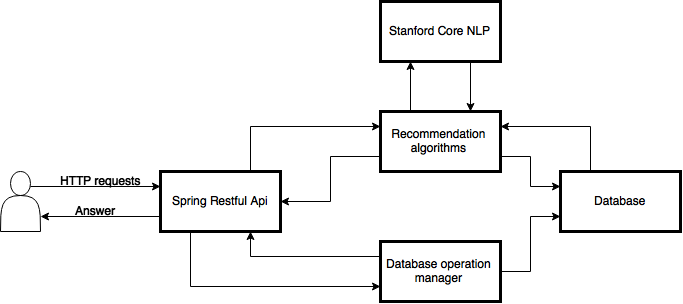
\includegraphics[width=1.0\textwidth]{src/img/architecture.png}
\end{figure}

\subsection{Programming languages}
\label{sec:programming-languages}
There were a multitude of programming languages to chose from.
In the following subsections we are going to discuss what languages we chose, why and for what purpose.

\subsubsection{Java}
\label{sec:programming-languages-java}
Java is a general purpose language that is class based, object oriented and concurrent. 
It is designed to have as few implemmentation dependencies as possible and be a "write once, run anywhere" type of language, meaning that compiled java code can run on all platforms that support java, without the need of recompilation.
Java applications are typically compiled to bytecode that can run on any Java virtual machine (JVM) regardless of the computer architecture.
\\ It is a language that supports multiple paradigms, as:  object-oriented, structured, imperative, functional, generic, reflective, concurrent. In our implemmentation we used the imperative, object-oriented and concurrent paradigms. By combining the object-oriented and imperative paradigms we managed to obtain a well structured and easy to read code base. By using the concurrent paradigm we are taking full advantage of the current multi-core arhitectures.
\\ Another reason for choosing Java is the great community and documentation. At the time of writing this document, Java was the most used language in the industry. Due to this, we can easily find support and documentation on any framework and problem we may stumble upon during the implemmentation of this system. Also, a great variety of frameworks exist for this language.


\subsubsection{Javascript}
\label{sec:programming-languages-javascript}
Javascript is a high level, dynamic, untyped and interpreted programming language. Alongside CSS and HTML, Javascript is one of the pillars of the current World Wide Web. In the last couple of years it has gained a great popularity in the detriment of action script, which was a programming language for the Adobe Flash Player. This movement towards Javascript is also because most mobile devices do not support Adobe Flash Player.
\\ Even though, Javascript may also be used as a backend programming language, since the launch of Node.js, which is  an open source, cross-platform runtime environment for server-side and networking applications, the most commonly usage of Javascript is as a client side scripting language. This means that the Javascript code is send along with the HTML to the browser, which then interprets it. A great advantage is the fact that the execution of the javascript code is done on the client, thus, in order to use it you just need to serve a file to the client.
\\ In our implemmentation we used Javascript and Node.js to create a demo application which easily integrates with our Recommender System. Javascript was used to create the graphical user interface, since we have an abundance of frameworks that enable us to create a quick and beautiful user interface. Because of various security issues, Javascript is not allowed to make cross domain requests, so Node.js was used in order to create a proxy between our Recommender System and the Javascript client. Also, Node.js was used to serve the files to the client.
\\ Also, in order to better show our Recommender System's capabilities, a Chrome plugin was built that could easily integrate with Adobe's existing platform.
\\ Since, Javascript is one of the pillars of the World Wide Web and our Recommender System was meant to easily integrate with a web application, Javascript was the first choice for our demo applications.


\subsection{Frameworks}
\label{sec:frameworks}
The main reason for using a framework is because we do not want to reinvent the wheel
\begin{itemize}
	\item Present Spring and why we chose it	
	\item Present Java and why use chose it
	\item Present HBASE and why we chose it( not sure about this. Small presentation in database design. Can bring it from there)
	\item Present Stanford lemmatizer and why we chose it.	
\end{itemize}


\section{Recommendation System Workflow} 
\label{sec:workflow}

\begin{itemize}
	\item Add the workflow
	\item Add all the workflows(use cases) and explain them in depth
\end{itemize}